\documentclass[14pt,a4paper]{scrartcl}

\usepackage[utf8]{inputenc}
\usepackage[english,russian,ukrainian]{babel}
\usepackage{indentfirst}
\usepackage{misccorr}
\usepackage{graphicx}
\usepackage[usenames,dvipsnames]{xcolor}

\usepackage{cmap}

\usepackage{amsmath,amsfonts,amssymb,amsthm,mathtools}
\usepackage{icomma}
\usepackage{multirow}
\usepackage{geometry} \geometry{verbose,a4paper,tmargin=1cm,bmargin=2.5 cm,lmargin=2cm,rmargin=1cm}
\usepackage{euscript}
\usepackage{hyperref}
\usepackage{mathrsfs}
\usepackage{mathtext}
\usepackage{graphicx}
\usepackage{booktabs}
\usepackage{color}
\usepackage{rotating}
\usepackage{pdflscape}
\usepackage{floatrow}
\usepackage{subcaption}
\usepackage{calc}
\usepackage{tikz}
\usepackage{fontawesome5}
\usetikzlibrary{shapes.geometric, arrows}
\usepackage[siunitx]{circuitikz}

\usepackage{listings}

\linespread{1.3}
\setlength{\parindent}{5ex}


\begin{document}

\pagecolor{white}
\begin{titlepage}
  \begin{center}
    \large
    Національний технічний університет України \\ "Київський політехнічний інститут імені Ігоря Сікорського"
     
       
    Факультет Електроніки
     
    Кафедра мікроелектроніки
    \vfill
      
    
     
    {\Large Домашня контрольна робота\\
      з дисципліни: «Мікропроцесори та мікроконтролери»
      }\\

	{\bf Секундомір}


  \bigskip
\end{center}
\vfill
 
\newlength{\ML}
\settowidth{\ML}{«\underline{\hspace{0.4cm}}» \underline{\hspace{2cm}}}
\hfill
\begin{minipage}{1\textwidth}
Виконав:\\
Студент 4-го курсу \hspace{4cm} $\underset{\text{(підпис)}}{\underline{\hspace{0.2\textwidth}}}$  \hspace{1cm}Мнацаканов А.С.\\
\vspace{1cm}

Перевірив: \hspace{6.1cm} $\underset{\text{(підпис)}}{\underline{\hspace{0.2\textwidth}}}$  \hspace{1 cm}Татарчук Д.Д.\\

\end{minipage}

\vfill

\begin{center}
2021
\end{center}
\end{titlepage}


\section*{\textrm{1. Мета роботи}}

Розробити секундомір

\section*{\textrm{2. Розробка схеми}}

Все що нам потрібно для секундоміра - це те, куди ми могли б виводити інформацію. Найкращим рішенням було використати символьний дисплей 1602 з інтерфесом I2C. Взагалі нам потрібно виводити лише цифри, для цього підійшов би і чотирьохрозрядний семисегментний індикатор а також здвиговий регістр 74HC595, але перший варіант найпростіший. Формуємо схему: 

\begin{figure}[!h]\TopFloatBoxes\CenterFloatBoxes
\ffigbox{\caption{Сформована схема для секундоміра.}}
{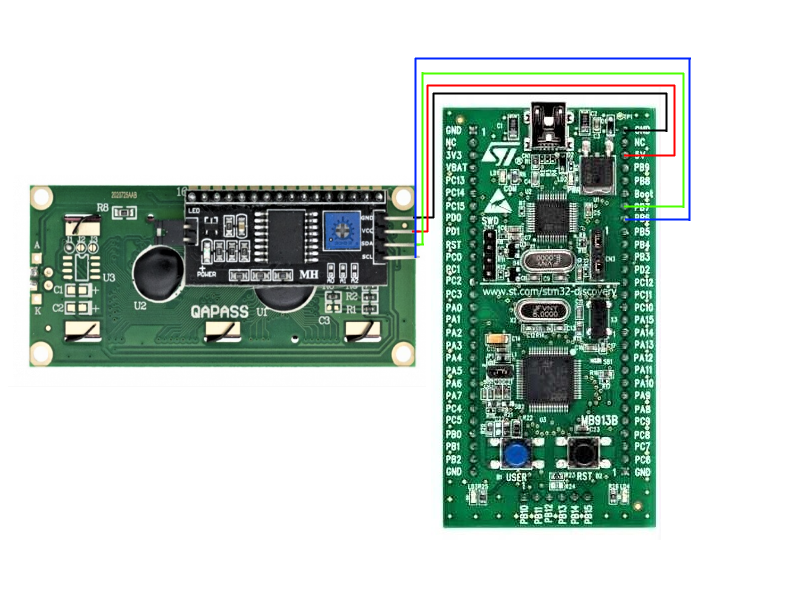
\includegraphics[scale=0.8]{shema.png}}
\end{figure}

\newpage

\section*{\textrm{3. Створення проекту}}

Піни PB7 та PB6 відповідають за лінії SDA та SCL. У розділі System Core: RCC обираємо пункт High Speed Clock (HSE)$\boxed{Crystal Ceramic Resonator}$. Також налаштуємо кнопку як цифровий вхід. Будемо зчитувати її положення - якщо на неї натиснути - висвітиться результат і відлік почнеться спочатку.

\begin{figure}[!h]\TopFloatBoxes\CenterFloatBoxes
\ffigbox{\caption{Налаштування ніжок мікроконтролера.}}
{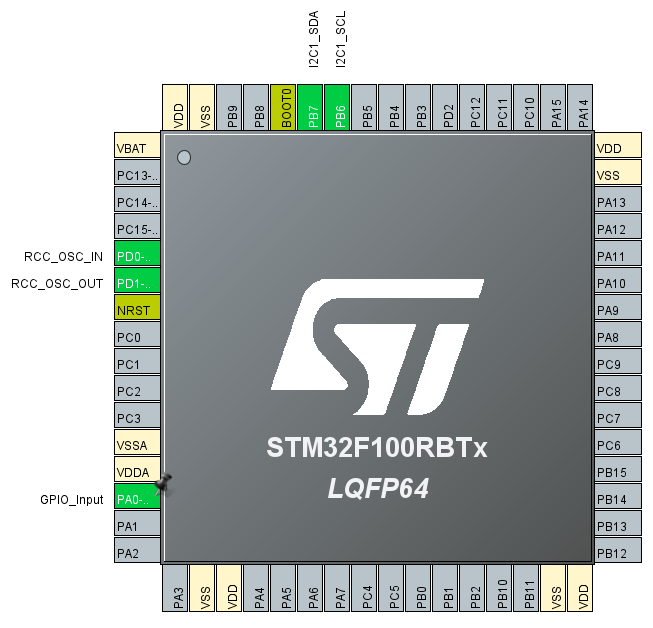
\includegraphics[scale=0.5]{pinout.png}}
\end{figure}


\begin{figure}[!h]\TopFloatBoxes\CenterFloatBoxes
\ffigbox{\caption{Налаштування тактування.}}
{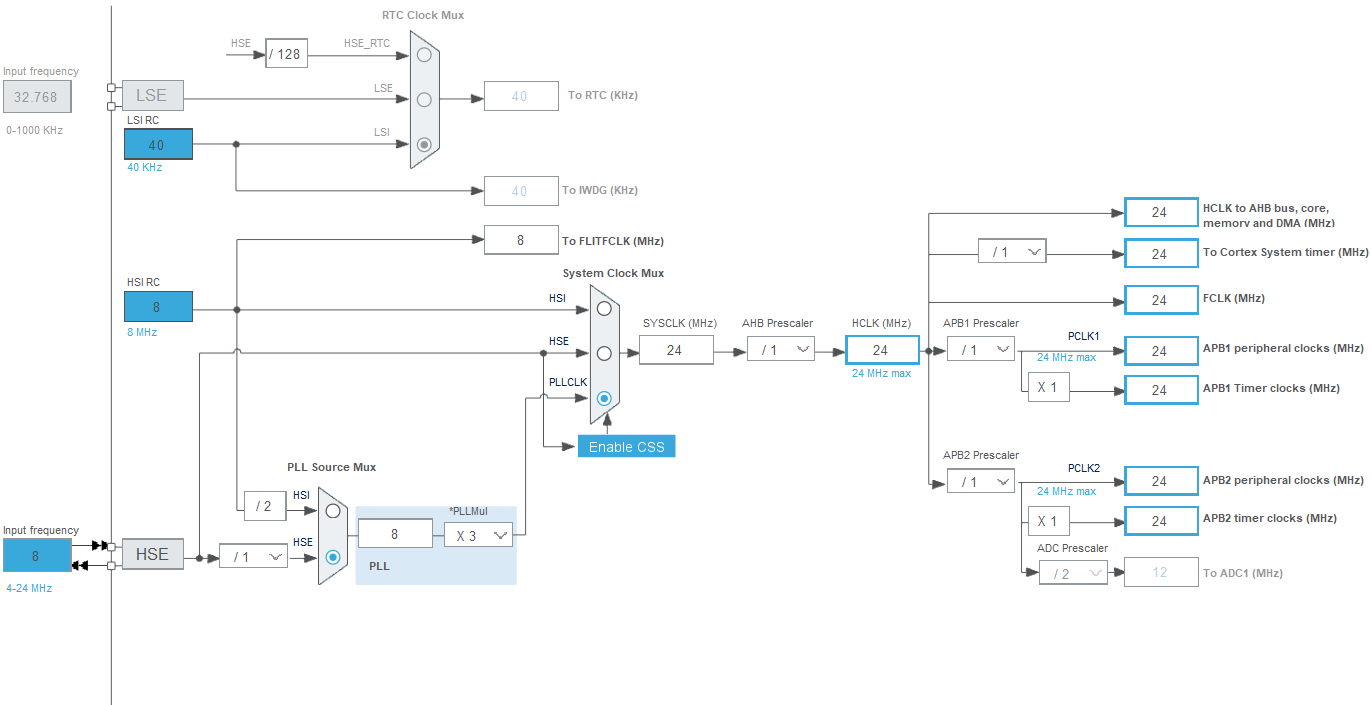
\includegraphics[scale=0.5]{clock.png}}
\end{figure}


\newpage
\section*{\textrm{5. Програмна частина}}

Розпишемо яка частина коду за що відповідає.


\lstset{
backgroundcolor = \color{red!10},
    tabsize=4,    
%   rulecolor=,
    language={C++},
escapechar={|},
        captionpos = t,
        basicstyle = \footnotesize\ttfamily,
        frame=lines,
        numbersep=5pt,
        numbers=left,
        numberstyle=\tiny,
        backgroundcolor=\color{red!5},
        aboveskip={1.5\baselineskip},
        columns=fixed,
        extendedchars=false,
        breaklines=true,
%        prebreak = \raisebox{0ex}[0ex][0ex]{\ensuremath{\hookleftarrow}},
        frame=single,
        showtabs=false,
        showspaces=false,
        keepspaces = true   %!!!! пробелы в комментариях
}


\begin{lstlisting}

/* USER CODE END Header */
/* Includes ------------------------------------------------------------------*/
#include <main.h>
#include <stdio.h>
#include <lcd1602_i2c_lib.h>
#include <math.h>

extern char lcd1602_tx_buffer[80]; //|\color{YellowGreen}\ttfamily создаём глобальный буфер данных|

int k;  //|\color{YellowGreen}\ttfamily переменная-счётчик|
int min;
int sec;

/* |\color{YellowGreen}\ttfamily две вспомогательные переменные для обработчика кнопки|*/
int prev_state = 0 ;
int current_state = 0 ;




/* Private includes ----------------------------------------------------------*/
\end{lstlisting}


\begin{lstlisting}
/* USER CODE BEGIN WHILE */
  while (1)
  {

	current_state = HAL_GPIO_ReadPin(GPIOA, GPIO_PIN_0) ; //|\color{YellowGreen}\ttfamily счит. тек-е состояние кнопки|

	  if ( ( prev_state == 0 ) && ( current_state != 0 ) ) //|\color{YellowGreen}\ttfamily если нажали|
	  {
		  lcd1602_Clean(); //|\color{YellowGreen}\ttfamily очищаем дисплей|

		  if(k>=60) //|\color{YellowGreen}\ttfamily если счётчик больше минуты - выполняем преобразования в мин. и сек.|
		  {
			  min = k/60;
			  sec = k

			  lcd1602_SetCursor(0,1);
			  sprintf(lcd1602_tx_buffer, "%d m,", min);
			  lcd1602_Print_text(lcd1602_tx_buffer);

			  lcd1602_SetCursor(5,1);
			  sprintf(lcd1602_tx_buffer, "%d s,", sec);
			  lcd1602_Print_text(lcd1602_tx_buffer);

		  }

		  else //|\color{YellowGreen}\ttfamily если нет, то просто выводи результат в секундах|  
		  {
			  sec = k % 60;

			  lcd1602_SetCursor(0,1);
			  sprintf(lcd1602_tx_buffer, "0 m,", min);
			  lcd1602_Print_text(lcd1602_tx_buffer);

			  lcd1602_SetCursor(5,1);
			  sprintf(lcd1602_tx_buffer, "%d s,", sec);
			  lcd1602_Print_text(lcd1602_tx_buffer);
		  }

		  k=0;
		  HAL_Delay(3000);
		  lcd1602_Clean();
	  }

	  else  //|\color{YellowGreen}\ttfamily если кнопку не трогаем, счётчик растёт и высвечивается на дисплее|
	  {
		  lcd1602_SetCursor(0,0);
		  sprintf(lcd1602_tx_buffer, "Time: %d s", k);
		  lcd1602_Print_text(lcd1602_tx_buffer);
		  HAL_Delay(1000);

		  k++;
	  }

	  prev_state = current_state ; //|\color{YellowGreen}\ttfamily возвращаем кнопку в неактивное состояние|


    /* USER CODE END WHILE */

    /* USER CODE BEGIN 3 */
  }
  /* USER CODE END 3 */
\end{lstlisting}





%%//|\color{YellowGreen}\ttfamily переменная, влияющая на коэффициент заполения|


% \href{https://youtu.be/Ovs5Fp5RFgY}{\textcolor{red}{тут}}.


%\begin{figure}[!h]\TopFloatBoxes\CenterFloatBoxes
%\ttabbox[\FBwidth+3cm]{\caption{Результати вимірювання передавальної характеристики $U_2=f(U_1)$ перемикача напруги на біполярному транзисторі для різних модифікацій схеми.}}
%{


%}
%\end{figure}


%\begin{figure}[!h]
% \ffigbox{\caption{My Caption}}
% {\includegraphics{roman_a}}
%\end{figure}

\end{document}